\chapter{De l’évolution des paysages \textit{cis}-régulateurs à l’évolution phénotypique : étude de la perte convergente du phallus chez les oiseaux}
{\hypersetup{linkcolor=GREYDARK}\minitoc}
\label{chap:4-evolpheno}

\section{Introduction}

Les adaptations morphologiques se mettent généralement en place durant le développement embryonnaire des individus et font intervenir des gènes contrôlant la différenciation cellulaire, la croissance et la régionalisation des différentes parties du corps. Ces gènes sont impliqués dans de nombreux processus biologiques et sont alors hautement pléiotropiques, ce qui contraint l’évolution de leur séquence codante. Les mutations qui affectent la séquence protéique codée par ces gènes ont souvent d'importantes conséquences et sont donc délétères pour l’organisme. Il est ainsi théoriquement attendu que la part des mutations dans les séquences codantes soit bien plus faible que celle des mutations dans les séquences non-codantes pour expliquer des changements morphologiques majeurs impliquant de tels gènes \glspl{pleiotrope} \citep{wray_evolutionary_2007, carroll_evo-devo_2008}. Des variations temporelles ou spatiales de l’expression des gènes seraient en mesure d’expliquer une part importante des changements évolutifs de la morphologie. Par exemple, des populations isolées d’épinoches présentent une réduction convergente de la ceinture pelvienne \citep{shapiro_genetic_2004}. Ce phénotype est principalement déterminé par l’expression du facteur de transcription \textit{Pitx1}, qui est impliqué dans le développement de nombreuses structures chez les vertébrés et qui est sous forte sélection purifiante. Les variations morphologiques observées chez les épinoches sont probablement le résultat de mutations dans des éléments \gls{cis}-régulateurs de \textit{Pitx1}, spécifiquement actifs dans ce tissu \citep{chan_adaptive_2010, thompson_novel_2018}. L’évolution des paysages \gls{cis}-régulateurs des gènes peut ainsi participer à des changements morphologiques importants. Les approches de génomique comparative combinées avec des annotations fonctionnelles permettent alors d’identifier les déterminants génétiques qui sont associés à l’évolution d’un phénotype. Détecter la présence, l’absence, l’activité et mesurer le taux d’évolution des éléments \gls{cis}-régulateurs peut ainsi permettre d’identifier les mécanismes responsables de changement d’expression des gènes à l’origine des variations phénotypiques. \\

Les causes génétiques ayant provoqué un changement phénotypique peuvent être difficiles à identifier, particulièrement lorsque celui-ci est ancien. Les pertes phénotypiques sont intéressantes de ce point de vue car quelle que soit la mutation initiale, il est attendu d’observer un relâchement des pressions de sélection purifiante sur les séquences impliquées exclusivement dans le développement et le maintien de ces caractères \citep{hiller_forward_2012, roscito_phenotype_2018}. Si ces séquences ne sont pas \glspl{pleiotrope}, elles deviennent non-fonctionnelles et évoluent alors de façon neutre. La présence d’une accumulation de mutations ou plus généralement du changement de taux d’évolution d'une séquence fournissent ainsi des indices sur son rôle dans le phénotype ancestral. Les cas de convergence évolutive, dans lesquels plusieurs lignées évoluent indépendamment vers des traits similaires, permettent d’étudier la répétabilité d’un processus évolutif \citep{sackton_convergent_2019}. Les lignées ayant perdu de manière convergente un trait phénotypique présentent ainsi une augmentation parallèle de la divergence sur les séquences impliquées dans ce trait par rapport à leur état ancestral. En analysant les taux d’évolution des gènes codants chez les mammifères, il a par exemple été montré que plusieurs gènes codant pour des récepteurs olfactifs présentent une accélération significative spécifique chez les espèces marines où les sens du goût et de l’odorat sont fortement réduits \citep{chikina_hundreds_2016}. En cherchant à comprendre les mécanismes moléculaires à l’origine de la perte convergente du vol chez les oiseaux, Sackton et collaborateurs n’ont quant à eux pas observé de taux d'évolution convergent dans les séquences codantes \citep{sackton_convergent_2019}. Cependant, grâce à des alignements de génomes complets, il est possible d’effectuer des comparaisons des taux d’évolution à l’échelle génomique et ainsi de cibler des régions non-codantes présentant des patrons d’évolution convergents en tenant compte des relations phylogénétiques entre espèces \citep{hiller_forward_2012,prudent_controlling_2016, partha_robust_2019}. Avec une telle approche, Sackton et collaborateurs ont détecté des accélérations convergentes des séquences de nombreux éléments \gls{cis}-régulateurs potentiels présentant des marques de chromatine ouvertes lors du développement des membres antérieurs de plusieurs oiseaux \citep{sackton_convergent_2019-1}. De même, en analysant les séquences non-codantes conservées à l’échelle de 24 espèces de vertébrés, Roscito et collaborateurs ont montré que plusieurs milliers de régions ont des taux d’évolution accélérés et convergents chez 4 espèces ayant un mode de vie souterrain \citep{roscito_phenotype_2018}. Plusieurs d’entre elles sont situées dans les promoteurs ou proches des gènes liés au développement ou ayant des fonctions relatives aux yeux, ce qui est cohérent avec la forte régression de cet organe chez les espèces souterraines.\\

Finalement, il est possible d’identifier si des pressions de sélection partagées ont produit des phénotypes similaires à partir de bases moléculaires identiques, faisant intervenir des mutations similaires sur les mêmes gènes ou éléments \textit{cis}-régulateurs. Par exemple, peu de séquences présentent une accélération du taux d’évolution convergent entre les serpents et deux espèces de lézards ayant perdu leurs membres (Figure \ref{fig:chap4-fig1}) \citep{roscito_convergent_2022}. La divergence d’éléments \gls{cis}-régulateurs distincts aurait impacté les patrons d’expression de gènes impliqués à plusieurs étapes dans la voie de signalisation du développement des membres. La potentielle pléiotropie des éléments \gls{cis}-régulateurs de ces gènes du développement pourraient maintenir une sélection purifiante suffisante sur leurs séquences pour ne pas observer de lien avec la perte phénotypique. De plus, les deux espèces de lézards semblent avoir perdu leurs membres relativement récemment par rapport aux serpents, ce qui pourrait ne pas avoir laissé suffisamment de temps pour observer une divergence de l’ensemble des séquences impliquées dans ce phénotype.

\begin{figure}[hbt!]
 \centering
 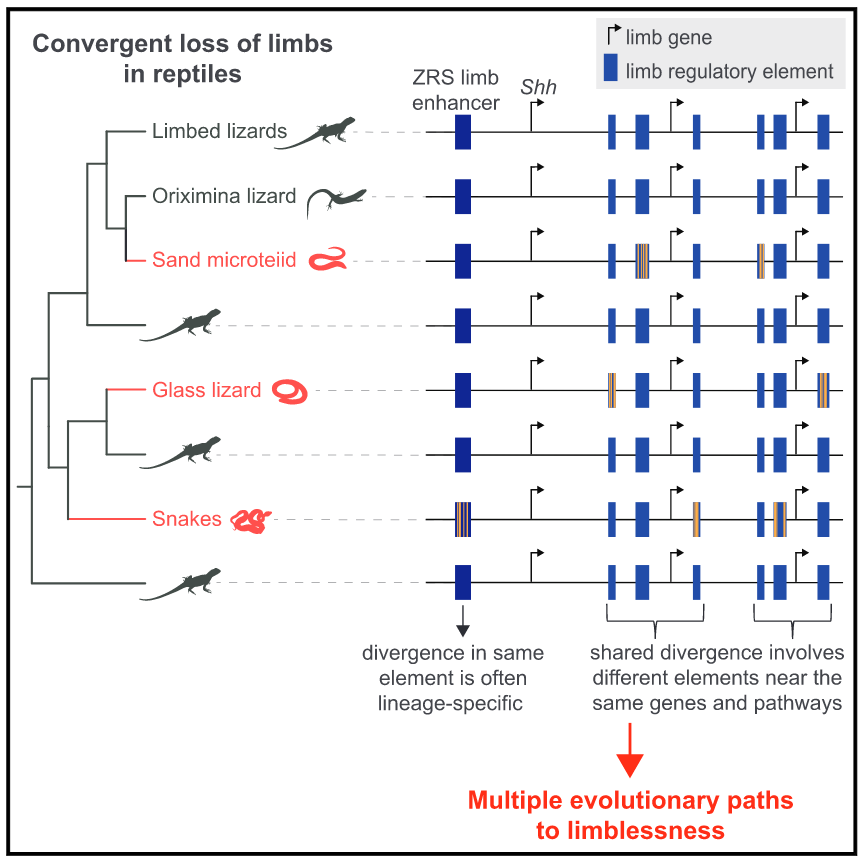
\includegraphics[width=0.7\textwidth, page=1]{figures/IPLOSS/chap4_Fig_intro.png}
 \caption[Évolution des séquences \gls{cis}-régulatrices en lien avec la perte convergente des membres chez les reptiles.]{
 \textbf{Évolution des séquences \gls{cis}-régulatrices en lien avec la perte convergente des membres chez les reptiles.} Les espèces ayant perdu les membres sont indiquées en rouge dans l'arbre phylogénétique. L'alignement de leurs génomes permet d'analyser l'évolution des séquences \gls{cis}-régulatrices (rectangles bleus) potentiellement impliquées dans la perte phénotypique convergente. Chez les serpents de nombreuses mutations (jaune) dans l'\gls{amplificateur} ZRS du gène \textit{SHH} sont associées avec cette perte phénotypique. Chez les deux autres espèces de lézard, la séquence de ZRS ne présente pas de mutations particulières par rapport aux espèces qui possèdent des membres. Les séquences de nombreux autres éléments \gls{cis}-régulateurs proches des gènes exprimés normalement dans le développement des membres (flèches noires) ont subi une accélération des taux d'évolution chez les espèces ayant perdu les membres. Des éléments \gls{cis}-régulateurs différents sont divergents selon les espèces mais sont présents autour des gènes impliqués dans les mêmes voix métaboliques. Tirée de \citet{roscito_convergent_2022}.
 \\
 }
 \label{fig:chap4-fig1}
\end{figure} 

\section{\'Etude de la perte convergente du phallus chez les oiseaux}
\label{sec:evol-phallus}

Au cours de ma thèse je me suis intéressé à l’évolution convergente du développement du phallus chez les oiseaux. Cet organe est présent chez l’ancêtre des amniotes mais a été réduit ou perdu dans plusieurs lignées d’oiseaux ainsi que chez une espèce de lézard, le tuatara \citep{brennan_independent_2008, sanger_resurrecting_2015}. Chez les oiseaux, plusieurs événements indépendants de réduction ou perte se seraient produits, notamment dans la lignée des Neoaves qui représente plus de 97\% de la diversité actuelle des oiseaux (Figure \ref{fig:chap4-fig-herrera}) \citep{brennan_independent_2008, feng_dense_2020}.\\

\begin{figure}[hbt!]
 \centering
 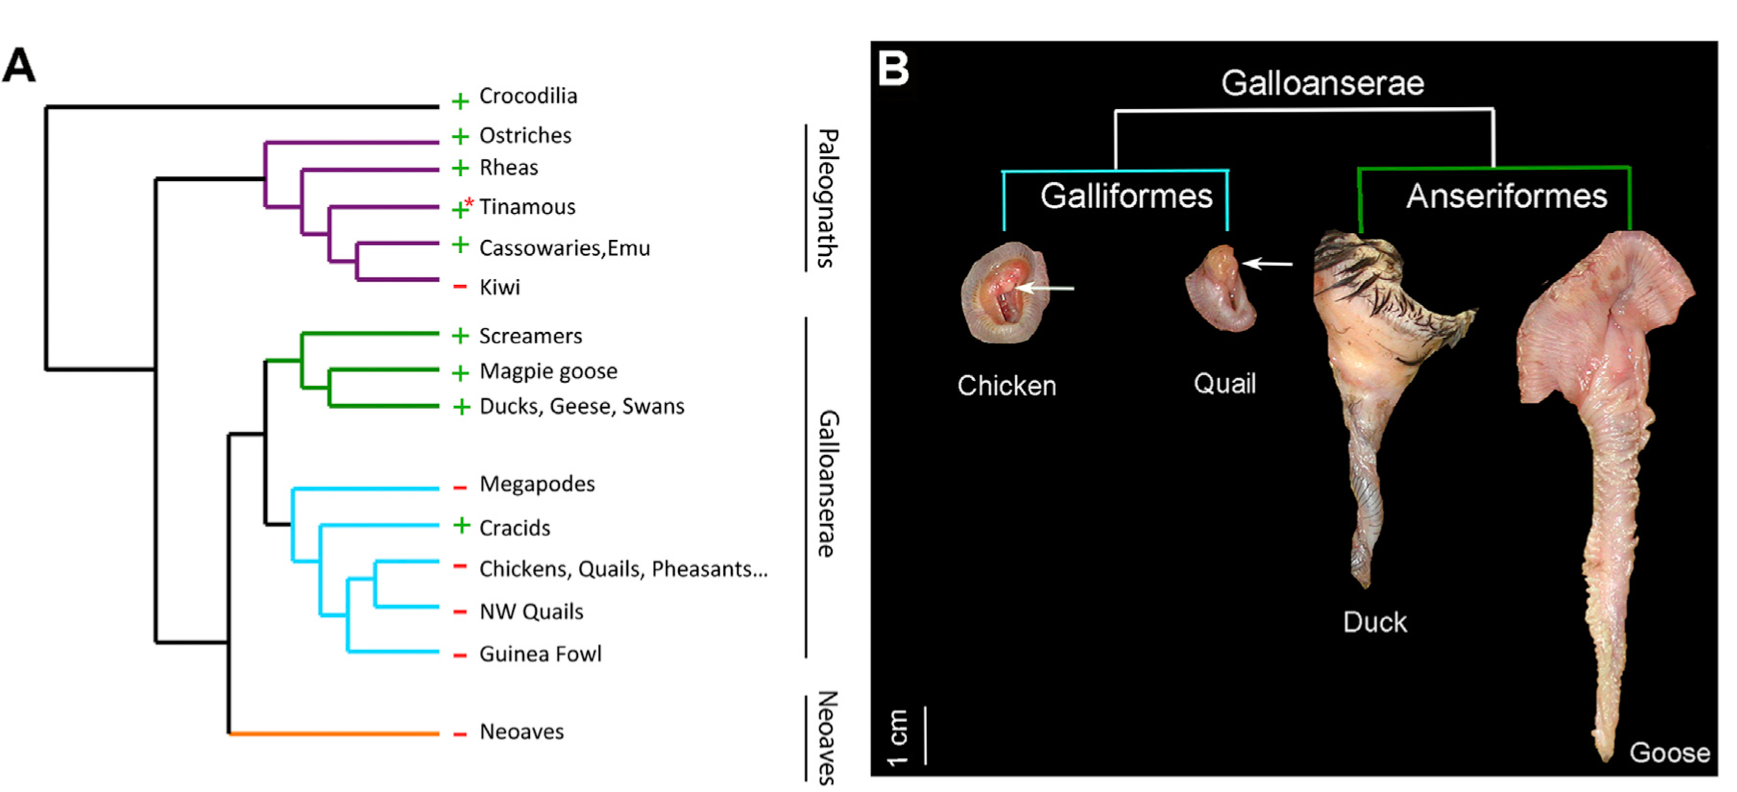
\includegraphics[width=1\textwidth, page=1]{figures/IPLOSS/Herrera2013_fig1.png}
 \caption[Pertes et réductions du phallus chez les oiseaux]{
 \textbf{Pertes et réductions du phallus chez les oiseaux}.
 \textbf{A.} Arbre phylogénétique représentant les grands groupes d'oiseaux. Les symboles "+" et "-" indiquent la présence ou l'absence (ou la réduction) du phallus chez le groupe d'espèces correspondant. 
 \textbf{B.} Morphologie du phallus à l'état adulte pour le poulet, la caille, le canard et l'oie.
 Tirée de \citet{herrera_developmental_2013}.
 \\
 }
 \label{fig:chap4-fig-herrera}
\end{figure} 

Plusieurs hypothèses évolutives non-exclusives ont été avancées pour expliquer ce changement morphologique majeur \citep{briskie_sexual_1997}. Une première propose que cette perte soit la conséquence d’une sélection sexuelle pour le choix du partenaire mâle. En effet, l’accouplement chez les espèces d’oiseaux ne possédant pas de phallus nécessite une importante coopération de la femelle pour faire interagir les cloaques des deux individus. Le cloaque est l’orifice postérieur qui est chez ces espèces la seule ouverture commune pour les voies reproductives, digestives et urinaires. La seconde hypothèse avance ainsi que la perte du phallus pourrait être lié à une sélection naturelle pour réduire les risques de transmission sexuelle de pathogènes, qui pourrait être plus élevés lors d’une intromission \citep{briskie_sexual_1997}. Ce mode de reproduction sans phallus permet également une copulation rapide qui pourrait avoir été sélectionnée pour réduire les risques de prédation \citep{wesotowski_reduction_1999}.\\

Les processus développementaux de ce changement phénotypique sont eux aussi encore mal connus. Chez le poulet, espèce dont les mâles ne possèdent pas de phallus, il a été montré que le tubercule génital (\acrshort{TG}) se développe d’une manière similaire au canard à des stades embryonnaires précoces \citep{herrera_developmental_2013}. \`A un stade plus avancé, là où le \acrshort{TG} chez le canard continue de se développer pour former un phallus, la croissance du \acrshort{TG} chez le poulet s’arrête avant de subir une mort cellulaire. Ce processus pourrait être la conséquence de changements de patron d’expression de gènes. Une étude de plusieurs gènes candidats, connus pour être importants pour le développement du phallus chez la souris, a mis en évidence une différence entre poulet et canard pour le patron d'expression du gène \textit{BMP4} (Figure~ \ref{fig:chap4-fig-herrera-insitu-bmp}). Ce gène, dont les rôles dans la mort cellulaire ont été démontrés dans d'autres contextes \citep{marazzi_msx2_1997,trousse_bmp4_2001,de_paepe_bmp4_2019}, activerait l’apoptose dans le \acrshort{TG} chez le poulet \citep{herrera_developmental_2013}. Par contre, cette étude n'a révélé aucun autre changement important de patron d'expression parmi les autres régulateurs du développement des génitaux, comme \textit{HOXD13}, \textit{HOXA13} ou \textit{SHH} (Figure \ref{fig:chap4-fig-herrera-insitu-hoxd13}). \\

\begin{figure}[hbt!]
 \centering
 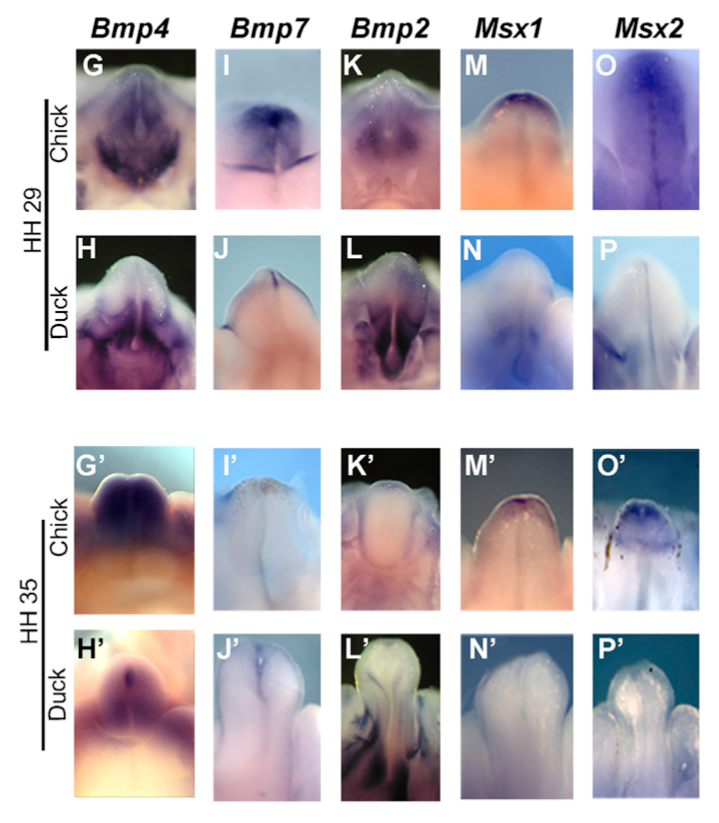
\includegraphics[width=0.8\textwidth, page=1]{figures/IPLOSS/Herrera2013_fig3.png}
 \caption[Patrons d'expression de gènes candidats au cours du développement du tubercule génital chez le poulet et le canard]{
 \textbf{Patrons d'expression de gènes candidats au cours du développement du tubercule génital chez le poulet et le canard}. 
 Ces graphiques représentent la distribution spatiale des produits des gènes \textit{BMP4}, \textit{BMP7}, \textit{BMP2}, \textit{MSX1}, \textit{MSX2} dans le tubercule génital de poulet ou de canard, à deux stades de développement (HH29 et HH35). L'expression des gènes a été évaluée avec des expériences d'hybridation \textit{in situ}. Le gène \textit{BMP4} présente un patron d'expression différent entre les TG du poulet et du canard au stade HH35.
 Tirée de \citet{herrera_developmental_2013}.
 \\
 }
 \label{fig:chap4-fig-herrera-insitu-bmp}
\end{figure} 

\begin{figure}[hbt!]
 \centering
 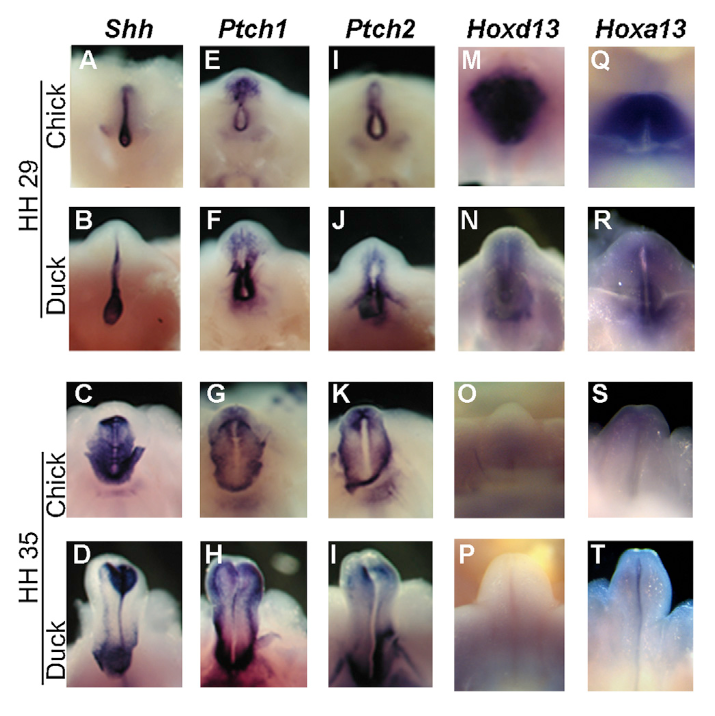
\includegraphics[width=0.8\textwidth, page=1]{figures/IPLOSS/Herrera2013_fig2.png}
 \caption[Patrons d'expression de gènes candidats au cours du développement du tubercule génital chez le poulet et le canard]{
 \textbf{Patrons d'expression de gènes candidats au cours du développement du tubercule génital chez le poulet et le canard}. 
 Ces graphiques représentent la distribution spatiale des produits des gènes \textit{SHH}, \textit{PTCH1}, \textit{PTCH2}, \textit{HOXD12}, \textit{HOXD13} dans le tubercule génital de poulet ou de canard, à deux stades de développement (HH29 et HH35). L'expression des gènes a été évaluée avec des expériences d'hybridation \textit{in situ}. Les gènes ne présentent pas de patrons différents de l'expression entre les deux espèces.
 Tirée de \citet{herrera_developmental_2013}.
 \\
 }
 \label{fig:chap4-fig-herrera-insitu-hoxd13}
\end{figure}

L'étude citée précédemment, qui est la première a avoir mis en évidence des patrons d'expression potentiellement en relation avec la réduction ou la perte du phallus chez les oiseaux, s'est concentrée sur une poignée de gènes candidats \citep{herrera_developmental_2013}. L'analyse de l'expression des gènes a été faite essentiellement de manière qualitative à l’aide d’hybridation \textit{in situ}. \`A ce jour, nous ne connaissons sans doute pas tous les changements d'expression des gènes qui pourraient être impliqués dans l'évolution de ce phénotype, ou qui pourraient survenir comme conséquence de l'évolution de ce phénotype. Pour étudier les mécanismes évolutifs et développementaux qui sont associés à ce changement phénotypique majeur, à l'échelle du génome entier, nous avons initié une collaboration avec Patrick Tschopp et Maëva Luxey de l’Université de Bâle en Suisse. Grâce à cette collaboration, nous avons pu combiner des analyses de données de transcriptomique et d'épigénomique à grande échelle avec des approches de génomique comparative, pour tenter de répondre à ces questions. Nous avons eu accès à des données de séquençage de \gls{transcriptome} (RNA-seq) pour 3 stades de développement comparables chez le poulet et le canard, ainsi qu'à des données de type ATAC-seq \citep{buenrostro_transposition_2013}, qui visent à identifier les régions de chromatine ouverte (dont les éléments \glspl{amplificateur}). \\

Dans un premier temps, nous avons ainsi étudié les variations des patrons de l’expression de l’ensemble des gènes codants orthologues entre le poulet et le canard au sein de plusieurs stades au cours du développement du tubercule génital. Deuxièmement, nous avons analysé l'activité des éléments régulateurs grâce aux données de type ATAC-seq. Nous devons noter ici que les données d'ATAC-seq dont nous disposons pour l'instant nécessitent d'être améliorées en termes de qualité. Nos collaborateurs sont à ce jour en train de générer une nouvelle série de données de ce type, qui devraient nous permettre de répondre à des questions plus approfondies sur l'activité des éléments \gls{cis}-régulateurs. Plutôt que d'attendre ces nouvelles données, nous avons exploité celles dont nous disposions déjà, mais en nous concentrant sur l'analyse de l'évolution de leurs séquences. Cette analyse ne devrait pas (ou peu) être affectée par les problèmes de qualité des données. Nous avons donc analysé les taux d’évolution des éléments \textit{cis}-régulateurs potentiels au sein de plusieurs lignées d’oiseaux. Nous avons évalué la corrélation entre les taux d'évolution dans chaque lignée avec la présence ou l’absence du phallus. Nous avons pour celà bénéficié des alignements de génomes complets publiés récemment par le consortium Birds 10K \citep{feng_dense_2020}, que nous avons complété avec quelques génomes supplémentaires. Nous notons également que notre objectif initial était d’utiliser des données de conformation de la chromatine (\acrshort{Hi-C}, disponibles pour plusieurs échantillons chez le poulet et chez le canard) pour associer les éléments régulateurs candidats avec leur gènes cibles. Cependant pour des contraintes de temps, nous avons pour l’instant utilisé une approche classique de voisinage. L’ensemble de ce travail n’est donc pas encore finalisé. La partie qui suit n’est ainsi que l’ébauche d’un article à partir des résultats que nous commençons à comprendre. \\

Finalement, dans le cadre de ce projet nous avons également séquencé et assemblé un génome brouillon pour le hocco à pierre (\textit{Pauxi pauxi}). Il s’agit d’un oiseau de la famille des Cracidés possédant un phallus et ayant une position phylogénétique intéressante pour l’étude de l’évolution de ce phénotype. Nous avons inclu cet oiseau dans les analyses présentées dans l’article suivant et nous avons souhaité détailler les caractéristiques de son génome, notamment grâce à des annotations en gènes et en éléments répétés, dans un travail présenté en Annexe (cf \ref{annexe:hocco}).
